% !TeX spellcheck = de_DE
\documentclass{uebung_cs}
\usepackage{algo223}
\uebung{1}{}{}

\blattname{Übungen zu Woche 1: Einführung und All Pairs Shortest Paths}
%%%%%%%%%%%%%%%%%%%%%%%%%%%%%%%%%%%%%%%%%%%%%%%%%%%%%%%%%%%%%%%%%%%%%%%%%%%%
\begin{document}

\begin{exercise}[Kennenlernen I][\atschool]
  Einführung.
\end{exercise}

\begin{exercise}[Kennenlernen II][\atschool]
  Wie heißt die Person neben dir?
  Was studiert sie?
  Was hat sie in den Ferien gemacht?
\end{exercise}

\begin{exercise}[Kennenlernen III][\atschool]
  Aufgaben sind meistens mit folgenden Emojis markiert:
  \begin{itemize}
    \item[\athome] Eigenständig \textbf{vor} dem nächsten Plenum bearbeiten (ca.~30 Minuten pro Aufgabe)
    \item[\atschool] Wird vorraussichtlich im Plenum bearbeitet und besprochen
    \item[\mittel] Eine mittelschwere Aufgabe (ca.~1 Stunde)
    \item[\note] Eine besonders schwere Aufgabe (mehrere Stunden)
    \item[\spass] Eine optionale Spaßaufgabe zum Knobeln
  \end{itemize}
\end{exercise}

\begin{exercise}[Telefonnetzwerk][\atschool\mittel]
  Wir betrachten die Schaltzentren eines Telefonnetzwerks sowie die Verbindungen zwischen diesen Schaltzentren.
  Die Verbindungen können zum Beispiel durch Kabel, Funk, oder Satellit realisiert werden.
  Wir assoziieren daher mit jeder Verbindung eine \emph{Bandbreite} und \emph{Kosten}.
  \begin{enumerate}
    \item Welches Konzept ist geeignet, um die Eingabe abstrakt zu modellieren?
    \item Gib einen Algorithmus an, der für zwei beliebige Schaltzentren $a$ und $b$ einen Verbindungsweg von $a$ nach $b$ ausrechnet, der die kleinsten Kosten verursacht.
    \item Die \emph{Bandbreite eines Verbindungsweg} ist die kleinste Bandbreite über alle einzelnen Verbindungen, die auf dem Weg auftauchen.
    Gib einen Algorithmus an, der für zwei Schaltzentren $a$ und $b$ einen Verbindungsweg von $a$ nach $b$ ausrechnet, der die größtmögliche Bandbreite hat.
  \end{enumerate}
\end{exercise}

\begin{exercise}[Mortys Labyrinth I][\atschool\athome]
  Morty muss einen stabilisierten Plumbus aus dem Klappen\-spitzen-Labyrinth beschaffen.
  Er muss dazu mit Ricks interdimensionaler \textit{portal gun} das Labyrinth betreten, durch das Labyrinth zu einem Plumbus vordringen, anschließend den (instabilen) Plumbus durch das Labyrinth zu einem Fleeb bringen, um ihn zu stabilisieren, und schließlich wieder zurück zum ursprünglichen Portal, um nach Hause zurückzukehren.
  Plumbusse werden durch Fleeb-Saft stabilisiert, der von jedem Fleeb abgesondert wird, sobald er aus seinem Fleeb-Loch entfernt wird.
  Instabile Plumbusse explodieren, wenn sie von ihrer Aufbewahrungs-Einheit über 137 Flinks weit getragen werden.
  Zudem stinkt das Klappenspitzen-Labyrinth nach Furz, weshalb Morty so wenig Zeit wie möglich dort verbringen will.

  Rick hat Morty für diese Aufgabe eine detaillierte Karte des Labyrinths gegeben, die aus einem gerichteten Graphen $G = (V,E)$ mit nicht-negativen Kantengewichten besteht (diese geben die Abstände in Flinks an).
  Zusätzlich hat er ihm die Menge $P \subseteq V$ der Plumbus-Aufbewahrungseinheiten und die Menge $F \subseteq V$ der Fleeb-Löcher mitgeteilt.
  
  Morty hat nun die Aufgabe, einen Startknoten $s \in V$, eine Plumbus-Aufbewahrungseinheit $p \in P$ und ein Fleeb-Loch $f \in F$ zu finden, sodass die Länge eines kürzesten Wegs von $p$ nach $f$ höchstens 137 Flinks beträgt und die Länge eines kürzesten Wegs, der von $s$ zunächst über $p$ und dann über $f$ schließlich zurück zu $s$ führt, so kurz wie möglich ist.

  Zeichne Mortys Problem in geeigneter Weise auf und beschreibe die Anforderungen anhand der Zeichnung.
\end{exercise}
\newpage
\begin{exercise}[Organisiert euch][\athome]
  \begin{enumerate}
    \item Wo findest du die Videos, wo die Übungsblätter, wo die alten Klausuren?
    Was passiert eigentlich im Plenum und was im Tutorium?
    Gibt es Bonuspunkte und wann ist die Klausur?
    All diese Informationen findest du auf der \href{https://tcs.uni-frankfurt.de/algo2/}{Webseite des Kurses} oder auf der \href{https://moodle.studiumdigitale.uni-frankfurt.de/moodle/course/view.php?id=5636}{Moodle-Seite des Kurses}.
    % , oder auf den \href{https://tcs.uni-frankfurt.de/algo2/ALGO2-Organisation.pdf}{Organisationsfolien}.
    Welche Fragen zum Kurs hast du jetzt noch? 
    \item Finde Mitstreiter:innen! Lernen macht mehr Spaß in der Gruppe. Wir empfehlen, dass ihr euch in Gruppen von 3-4 Personen organisiert. Trefft euch zum Anschauen der Videos und zum Lösen der Übungsaufgaben. Ihr könnt euch gegenseitig helfen, wenn ihr bei den Übungsaufgaben nicht weiterkommt. Und nach den Anstrengungen gemeinsam Tee trinken.
    \item Das ist der vermutlich schwierigste Kurs im B.Sc.~Informatik, rechne also damit, dass er viel Zeit in Anspruch nehmen wird.
    Erstelle für jede Woche im Semester einen detaillierten Wochenplan für dich und deine Lerngruppe. Entscheide, an welchen Angeboten von ALGO2 du wann teilnehmen möchtest. Zum Beispiel:
    \begin{itemize}
      \item\textbf{Inhaltlicher Input:} Falls ihr die Videos schauen wollt, plant ca.~2 Stunden mit Pausen, hitzigen Diskussionen, im Buch Nachlesen ein. Am Besten ein paar Tage vor dem Plenum. Nicht erst in der Nacht davor! Falls ihr ein Konzept nicht versteht, schaut mal in diesem Internet nach, oder ob es auf Youtube ein passendes Video dazu gibt.
      \item\textbf{Vorbereitende Übungsaufgaben:} Vor dem Plenum solltet ihr alle Übungsaufgaben und Teilaufgaben bearbeiten, die mit \athome markiert sind. Diese Aufgaben sind so gewählt, dass ihr sie auf Grundlage des inhaltlichen Inputs in eurer Lerngruppe eigenständig bearbeiten könnt. Wir erwarten nicht, dass ihr immer eine perfekte Antwort findet, aber falls ihr bei diesen Aufgaben regelmäßig gar keine Ahnung habt, müsst ihr unbedingt herausfinden, woran das liegt! Fehlen euch zum Beispiel Grundlagen aus einer vorherigen Vorlesung oder aus der Schule? Diese müsst ihr unbedingt nacharbeiten.
      \item\textbf{Plenum Dienstag und Donnerstag 8-10 Uhr:}
      Wir besprechen im Plenum kurz die Lösungen zu den \athome-Aufgaben.
      Danach geht es im Plenum um die mittelschweren bis schweren Lernziele und Übungsaufgaben.
      Die meiste Zeit werdet ihr in Gruppen unter Anleitung eines Dozenten an diesen Aufgaben arbeiten.
      \item\textbf{Nachbereitung und Projekte:}
      Ihr solltet euch detaillierte Notizen machen und die Übungsaufgaben fertig bearbeiten, am Besten schriftlich.
      Ihr habt auch die Möglichkeit, Übungsaufgaben eurer Wahl zu einem Projekt zu machen---hierzu reicht ihr eure möglichst fleißig ausgearbeitete Lösung bei eurem Tutor oder eurer Tutorin ein---er oder sie gibt euch dann detailliertes Feedback.
      Reicht lieber eine Lösung ein, an der ihr lange gearbeitet habt, als viele Lösungen, die ihr nur halbherzig bearbeitet habt.
      Falls das Feedback nicht nützlich war, überlegt euch, woran das gelegen haben könnte und sprecht das unbedingt im Tutorium an.
      \item\textbf{Tutorium:}
      Das Ziel des Tutoriums ist es, dir und deiner Lerngruppe möglichst individuelles und nützliches \textbf{Feedback} zu geben.
      Die meiste Zeit arbeitet ihr im Tutorium in Kleingruppen von 3-4 Personen zusammen an denjenigen Übungs- oder Klausuraufgaben, die ihr noch lösen möchtet (ihr sucht euch aus welche!).
      Das kann eine Aufgabe sein, von der ihr die Lösung noch nicht kennt.
      Oder auch eine, von der ihr die Lösung zwar schon gesehen habt (z.B. im Plenum), aber noch nicht ganz sicher damit seid.
      Ihr könnt auch während des Tutoriums eure Lösung schriftlich ausarbeiten. Schriftliche Ausarbeitungen könnt ihr eurem Tutor zeigen und ihr erhaltet dann mündliches und schriftliches Feedback darauf.
      \item\textbf{Lösungsspaziergänge:}
      Die Lösungsspaziergänge enthalten hübsch aufgearbeitete Lösungsideen zum Wohlfühlen.
      Die Lösungsspaziergänge sind nicht Teil des Tutoriums, sondern werden in den zwei Recap-Wochen anstatt des Plenums von Tutor:innen präsentiert.
    \end{itemize}
    \end{enumerate}
\end{exercise}

\newpage
\begin{exercise}[Coderunner ausprobieren][\emoji{hatching-chick}]
  Löse \enquote{Aufwärmübung: Coderunner ausprobieren} auf Moodle.
\end{exercise}

% \begin{exercise}[Pfannkuchensortierung]
%     Gegeben ist ein Stapel von $n$ Pfannkuchen verschiedener Größe.
%     Du musst die Pfannkuchen der Größe nach sortieren, sodass am Ende kleinere Pfannkuchen auf größeren Pfannkuchen liegen.
%     Die einzige erlaubte Operation ist ein \emph{flip}: Führe einen Pfannenwender unter die obersten $k$ Pfannkuchen für eine natürliche Zahl~$k$ ein und wende sie um.
%     \begin{enumerate}
%         \item Beschreibe einen Algorithmus, der einen beliebigen Stapel von $n$ Pfannkuchen mit $O(n)$ flips sortiert. Wie viele flips braucht dein Algorithmus im worst-case genau?
%         \item Für jede positive Zahl $n$, beschreibe einen Stapel mit $n$ Pfannkuchen, auf dem dein Algorithmus $\Omega(n)$ flips benötigt.
%     \end{enumerate}
% \end{exercise}

% \newpage
\begin{exercise}[APSP-Algorithmen Motivation][\athome]
  Löst nicht schon Dijsktra's Algorithmus das APSP-Problem?
  Warum brauchen wir besondere APSP-Algorithmen, wenn wir doch kürzeste Wege schon ausrechnen können?
  In welchen Anwendungen will man überhaupt jemals APSP ausrechnen, anstatt nur normale kürzeste Wege zwischen zwei Knoten?
  Inwiefern wäre es sinnvoll, umgekehrt die neuen APSP-Algorithmen zu nutzen, um damit einen kürzesten Weg zwischen zwei Knoten auszurechnen?
\end{exercise}

  \begin{exercise}[APSP-Algorithmen anwenden][\athome]
  Gegeben sei der gerichtete und gewichtete Graph~$G$ aus Abbildung~\ref{example_graph}.
  Führe den Algorithmus \textsc{FloydWarshall} [Erickson, Abschnitt~9.8] von Hand Schritt für Schritt auf $G$ aus. 
  Beginne, indem du dir eine $(5\times 5)$-Matrix über $\mathbb N\cup\{\infty\}$ aufmalst, die den Zustand des \texttt{dist[.,.]}-Arrays für $r=0$ enthält (also die Basisfälle).
  Zeichne danach jeweils den Zustand des Arrays nach den Iterationen $r=1,2,\dots,5$.

\begin{figure}[ht]
	\begin{center}
		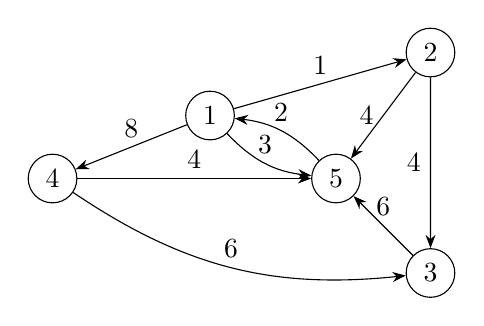
\begin{tikzpicture}[scale=0.8]
			\usetikzlibrary{arrows.meta}
%			\node[draw,circle] (v0)  at (0,  3.5)	{$6$};
			\node[draw,circle] (v1)  at (2.5,2.5)	{$1$};
			\node[draw,circle] (v2)  at (6,  3.5)	{$2$};
%			\node[draw,circle] (v3)  at (12, 3.5)	{$3$};
			\node[draw,circle] (v4)  at (0,1.5)	{$4$};
			\node[draw,circle] (v5)  at (4.5,1.5)	{$5$};
%			\node[draw,circle] (v6)  at (9,1.75)	{$6$};
%			\node[draw,circle] (v7)  at (12,1.75)	{$7$};
%			\node[draw,circle] (v8)  at (2.5,0)	{$6$};
			\node[draw,circle] (v9)  at (6,0)	{$3$};
%			\node[draw,circle] (v10) at (9,0)	{$7$};
%			\node[draw,circle] (v11) at (12,0)	{$11$};
			%
			\def\list {v1/v2/1, v1/v4/8, %v0/v1/6, v0/v2/4, v1/v5/3, v2/v3/6, v2/v6/8,
      v4/v5/4, %v4/v8/5, v8/v9/1,
      v9/v5/6%, v9/v10/4, v10/v7/7, v10/v11/2
      }  % list elements
			\foreach \u\v\weight in \list
			{	\draw[-Stealth] (\u) -- (\v) node [midway, above] {\weight};
			}
			\def\vertical {v2/v5/4, v2/v9/4%, v0/v4/3, v3/v7/7, v6/v10/1, v11/v7/2
      }  % list elements
			\foreach \u\v\weight in \vertical
			{	\draw[-Stealth] (\u) -- (\v) node [midway, left] {\weight};
			}
			
%      \draw[-Stealth] (v10) -- (v2) node [midway, above] {5};
      \path[-Stealth] (v5) edge[bend angle=20, bend right] node[above] {2} (v1);
      \path[-Stealth] (v1) edge[bend angle=20, bend right] node[above] {3} (v5);
      \path[-Stealth] (v4) edge[bend angle=20, bend right] node[above] {6} (v9);
		\end{tikzpicture}
		\caption{\label{example_graph}Der gerichtete, gewichtete Graph $G$. Die Zahlen an den Kanten definieren die Funktion $w\colon E(G)\to\mathbb N$ der Kantengewichte.}
	\end{center}
\end{figure}
\end{exercise}

\begin{exercise}[Backtracking in APSP-Algorithmen]
\ 
  \begin{enumerate}
    \item \athome
    Betrachte \textsc{LeyzorekAPSP} [Erickson, Abschnitt~9.6] und \textsc{FloydWarshall} [Erickson, Abschnitt~9.8].
    Welche Daten werden von diesen Algorithmen aufrecht erhalten?
    Was ist das Ergebnis am Ende der Berechnung?
    Welche Gemeinsamkeiten haben die beiden Algorithmen?
    Welche Unterschiede?
    Warum benutzen wir die Einträge $\infty$?
    \item \atschool Beschreibe, wie der Algorithmus \textsc{LeyzorekAPSP} [Erickson, Abschnitt~9.6] modifiziert werden kann, um neben dem Array der Längen kürzester Wege außerdem ein Array von Vorgänger-Pointern zurückzugeben.
    Die Laufzeit soll weiterhin in $O(V^3 \log V)$ liegen.
    \item \atschool Beschreibe, wie der Algorithmus \textsc{FloydWarshall} [Erickson, Abschnitt~9.8] modifiziert werden kann, um neben dem Array der Längen kürzester Wege außerdem ein Array von Vorgänger-Pointern zurückzugeben.
    Die Laufzeit soll weiterhin in $O(V^3)$ liegen.
  \end{enumerate}
  \emph{Hinweis zu b) und c)}: Das gesuchte Array \texttt{pred} ist ein zweidimensionales Array, das jedem Knoten-Paar $(u,v)$ einen Knoten \texttt{pred[u,v]} zuordnet. Hierbei soll \texttt{pred[u,v]} der Vorgänger-Knoten von $v$ auf einem kürzesten Weg von $u$ nach $v$ sein.
\end{exercise}

\begin{exercise}[Mortys Labyrinth II][\atschool]
  Beschreibe einen Algorithmus, um das Problem aus Mortys Labyrinth I zu lösen, und analysiere seine Laufzeit.
  Du darfst annehmen, dass eine Lösung existiert.
\end{exercise}

%\begin{exercise}
%  Die in der Vorlesung behandelten Algorithmen scheitern, sobald ein negativer Zyklus im Graph enthalten ist.
%  Sie können allerdings so modifiziert werden, dass sie auch im Falle von negativen Zyklen korrekte Längen kürzester Pfade berechnen.
%  Damit ist gemeint, dass im Fall, das entsprechende Array \texttt{dist} für ein Knotenpaar $u,v$ folgenden Wert enthalten soll:
%  \begin{itemize}
%  	\item Gibt es keinen $u$-$v$-Pfad im Graphen, dann soll $\texttt{dist}[u,v] = \infty$ sein.
%    \item Ist von $u$ ein negativer Zyklus erreichbar, von dem aus wiederum $v$ erreichbar ist, so soll $\texttt{dist}[u,v] = -\infty$ sein.
%    \item Andernfalls soll $\texttt{dist}[u,v]$ die Länge eines kürzesten $u$-$v$-Pfades angeben.
%  \end{itemize}
%  \begin{enumerate}
%    \item Zeige dies beispielhaft für den Floyd-Warshall-Algorithmus.
%    Beschreibe also, wie dieser modifiziert werden kann, um auch im Falle von negativen Zyklen korrekte Längen kürzester  Wege zu berechnen.
%    \item Zeige, dass der Floyd-Warshall-Algorithmus außerdem so modifiziert werden kann, dass er einen negativen Zyklus im Graphen zurückgibt, falls ein solcher existiert. Andernfalls soll weiterhin das Array der Längen kürzester Wege zurückgegeben werden.
%  \end{enumerate}
%\end{exercise}

\begin{exercise}[Puzzle der Woche: 99 Polizisten][\spass]
  In einer Stadt arbeiten 99 Polizisten.
  Jeder Polizist ist entweder ehrlich oder korrupt, wobei die Mehrheit der Polizisten ehrlich ist.
  Finde mit weniger als 299 Fragen heraus, welches die korrupten Polizisten sind.
  
  Dabei wissen alle Polizisten, welche der Polizisten ehrlich und welche korrupt sind, aber nur ehrliche Polizisten antworten immer wahrheitsgemäß.
  Korrupte Polizisten lügen möglicherweise.
  Aus sicherheitsgründen können nur Fragen folgenden Typs gestellt werden: Du kannst einen Polizisten X fragen, ob Polizist Y korrupt ist.
  Die Antwort darauf lautet entweder \enquote{Y ist korrupt} oder \enquote{Y ist ehrlich}.
\end{exercise}

\newpage
\section*{\projekt{} Projekte}

Bearbeite mit deiner Lerngruppe jede Woche mindestens ein \emph{Projekt}, stelle es im Tutorium vor und gib es bei deinem Tutor ab.
Du erhälst dadurch mündliches und/oder schriftliches Feedback vom Tutor und von anderen Studis.

\emph{Wann und mit wem soll ich das Projekt bearbeiten?}
Du entscheidest dich jede Woche spätestens im Tutorium für dein Projekt der Woche.
Such dir in deinem Tutorium Gleichgesinnte aus, die dasselbe oder ein ähnliches Projekt bearbeiten möchten.
Bearbeitet euer Projekt in einer Gruppe von maximal 4 Personen.
Die Zusammenstellung der Gruppen kann jede Woche neu sein.
Ihr fangt direkt im Tutorium an, an dem Projekt zu arbeiten.
Ihr schließt das Projekt im Laufe der folgenden Tage ab und gebt die schriftliche Ausarbeitung spätestens eine Woche später bei eurem Tutor ab.

\emph{Welches Projekt soll ich bearbeiten?}
Es ist völlig dir überlassen.
\emph{Echt jetzt?}
Du bist Expertin und Experte für dich und weißt am Besten, was du noch nicht kannst und was dir Spaß macht.
Das Projekt sollte etwas mit ALGO2 zu tun haben und weder zu einfach noch zu schwierig für dich sein. Siehst du den genauen Schritt-für-Schritt Ablauf schon vor deinem inneren Auge und bist sicher, dass du das auch wirklich problemlos umsetzen könntest, dann ist das Projekt zu einfach.
Wenn du auch nach 15 Minuten Überlegen gar keine Ahnung hast, wie du überhaupt anfängst und was du tun müsstest, dann ist das Projekt zu schwierig.
Wir sind gespannt, welche Projekte ihr euch überlegt!

\subsection*{Konkrete Projektideen für die aktuelle Woche}
\begin{itemize}
  \item
  Wähle eine oder mehrere Aufgaben vom aktuellen Übungsblatt aus und bearbeite sie schriftlich.
  \item
  Implementiere einen oder mehrere APSP-Algorithmen deiner Wahl in einer Programmiersprache deiner Wahl.
  Um zu prüfen, ob deine Implementierung korrekt ist, steht dir in Moodle ein Coderunner-Modul zur Verfügung, welches Python, C++, C und Java unterstützt.
  Lass deine Implementierung auf Eingabegraphen aus der echten Welt laufen.
  Bei \emph{Network Repository} (\url{https://networkrepository.com/}) gibt es tausende von Graphen, etwa Straßennetzwerke oder Gehirnbahnen.
  Wie groß darf der Graph sein, damit deine APSP-Berechnung noch in vernünftiger Zeit fertig wird?
\end{itemize}

\subsection*{Formale Anforderungen an die Projekte}
\begin{itemize}
  \item
  Nutzt dieses LaTeX-Template für eure schriftlichen Ausarbeitungen: \url{https://github.com/goethe-tcs/note-template}. Auch ein Link zu Overleaf findet sich dort, damit ihr direkt im Browser und ohne großes Vorwissen loslegen könnt.
  Wichtig ist, dass auf der Ausarbeitung eure Namen und eure \texttt{@stud.uni-frankfurt.de} E-Mail-Adresse stehen.
  Matrikelnummern sollen dort nicht stehen.
  \item
  Ganz wichtig ist, dass ihr am Anfang die Fragestellung wiederholt und erklärt. Was war die Übungsaufgabe oder das Problem, die oder das ihr gelöst habt?
  % \item
  Reflektiert in eurer Ausarbeitung außerdem kurz, wie schwierig ihr die Aufgabe fandet, wie lange ihr gebraucht habt und was ihr gelernt habt.
  \item
  Schreibt eure Lösung mit so vielen zusätzlichen Erklärungen, dass ihr sie problemlos nachvollziehen könnt, wenn ihr in zehn Jahren wieder drauf schauen würdet.
  Aber haltet euch dennoch kurz und entfernt alle Textteile, die nicht zur Lösung oder zum Verständnis beitragen.
  \item
  Wechselt jedesmal die Rollen in der Lerngruppe: Einer schreibt den ersten Textentwurf, eine redigiert---das heißt, sie liest das Geschriebene ganz kritisch und gibt Feedback---, eine editiert und korrigiert den Text. Jeder in der Lerngruppe sollte im Laufe des Semesters mal geschrieben haben, jeder sollte mal gegengelesen haben, jeder sollte mal editiert haben.
  \item
  Die Abgabe erfolgt dann im Tutorium als ausgedrucktes DIN-A4 Blatt oder in Absprache bei eurem Tutor per E-Mail als PDF-Datei.
  \item
  Feedback erhälst du auf deine schriftliche Ausarbeitung von deinem Tutor im Tutorium selbst.
  \item
  Jedes Projekt darf nur bei einem Tutor abgegeben werden!
\end{itemize}
\end{document}
